\newpage
\section{Context}
In this first section of the report, we will aim to provide the reader with a complete overview for the background of the project itself. Before introducing in detail every engineering aspect that lead the development, we will 

\subsection{Team description}
CHIC - Team descrition, goals, fieldwork

\vspace{1cm}
\begin{tabular}{m{2cm}m{5cm}m{2cm}m{5cm}}
    
    
\includegraphics[width=2cm]{images/icon_marjane.png} & \textbf{Marjane Amara} \newline Industrial Design &
    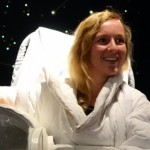
\includegraphics[width=2cm]{images/icon_chloe.jpg} & \textbf{Chloe Dickson} \newline Firmware Engineering \newline Mechanical Engineering \\
    
     & & & \\
    
    
\includegraphics[width=2cm]{images/icon_estelle.jpg} & \textbf{Estelle Geneux} \newline Business &
    
\includegraphics[width=2cm]{images/icon_yann.jpg} & \textbf{Matteo Yann Feo} \newline Software Engineering \\
    
     & & & \\
    
    
\includegraphics[width=2cm]{images/icon_simone.png} & \textbf{Simone Sanso} \newline Electronic Engineering \newline Firmware Engineering &
    
\includegraphics[width=2cm]{images/icon_luca.png} & \textbf{Luca Sassoli de Bianchi} \newline User Experience\\
\end{tabular}

\subsection{Product description}
Have you ever felt like spending more time with your children? Toygether is a plush toy for kids that connects to their parent’s smartphone. It enables parents to interact and play games with their children, even when far apart. Our plush toy features colourful lights and sounds to enhance the playing experience with children from 2 to 5 years old. With ever increasing working days and commute times, parents might have less time to spend with their loved ones. Toygether aims to bridge this gap by providing a screen-less interaction platform, enabling young children and parents to play together, even when they can’t physically be together.

\subsubsection{Interaction Design}
\label{sec:interaction_design}

\begin{figure}[H]
    \centering
    \subfloat[\label{fig:CHIC1}]{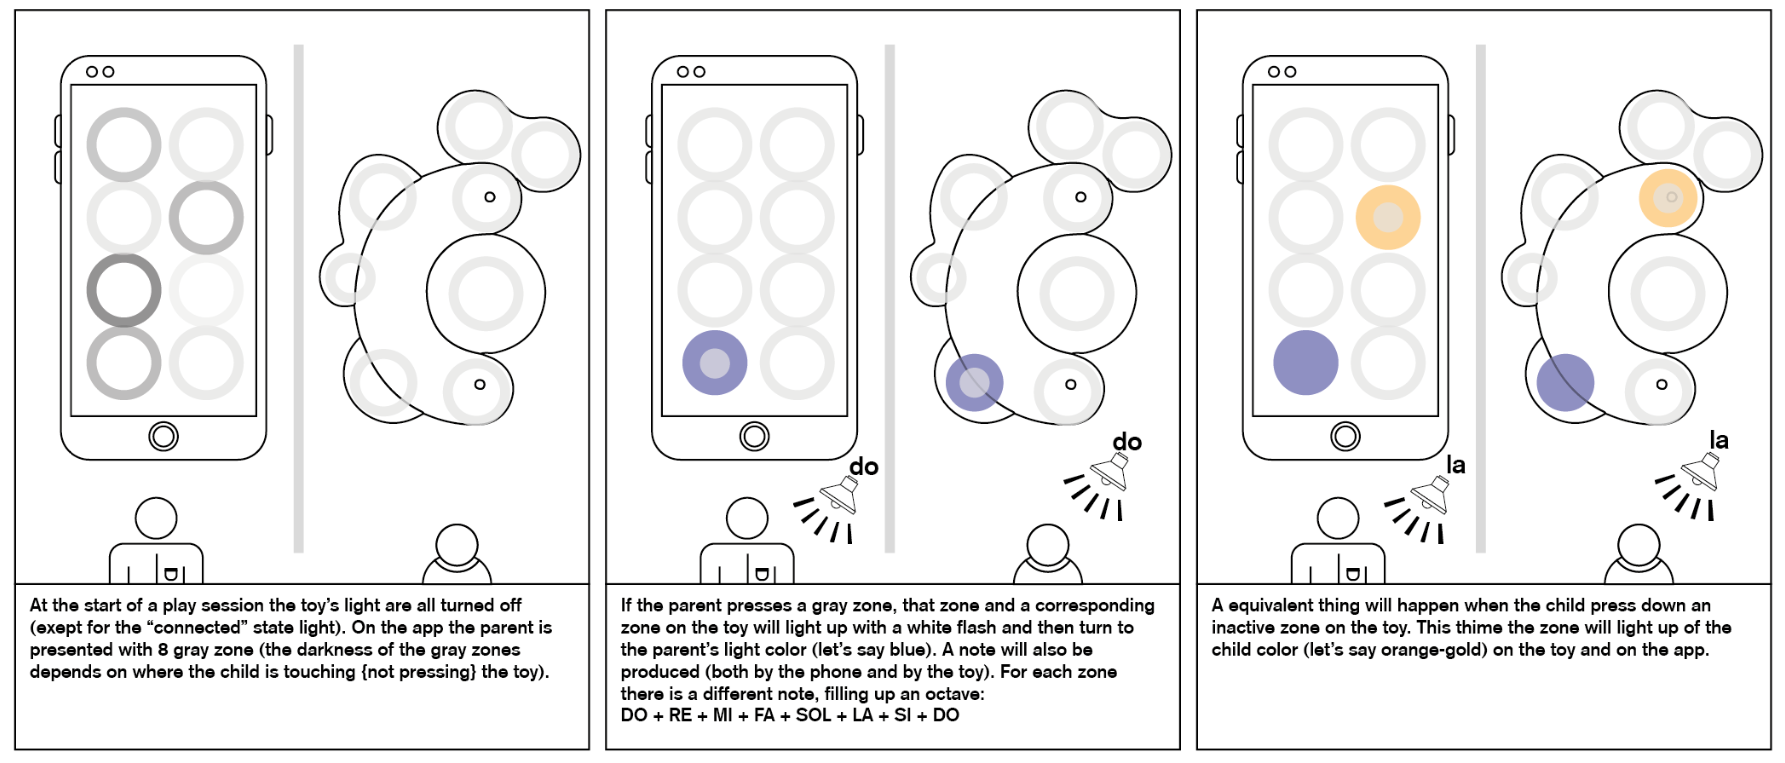
\includegraphics[scale=0.35]{images/FW/play_1.PNG}}\hfill
    \subfloat[\label{fig:APA102_1}] {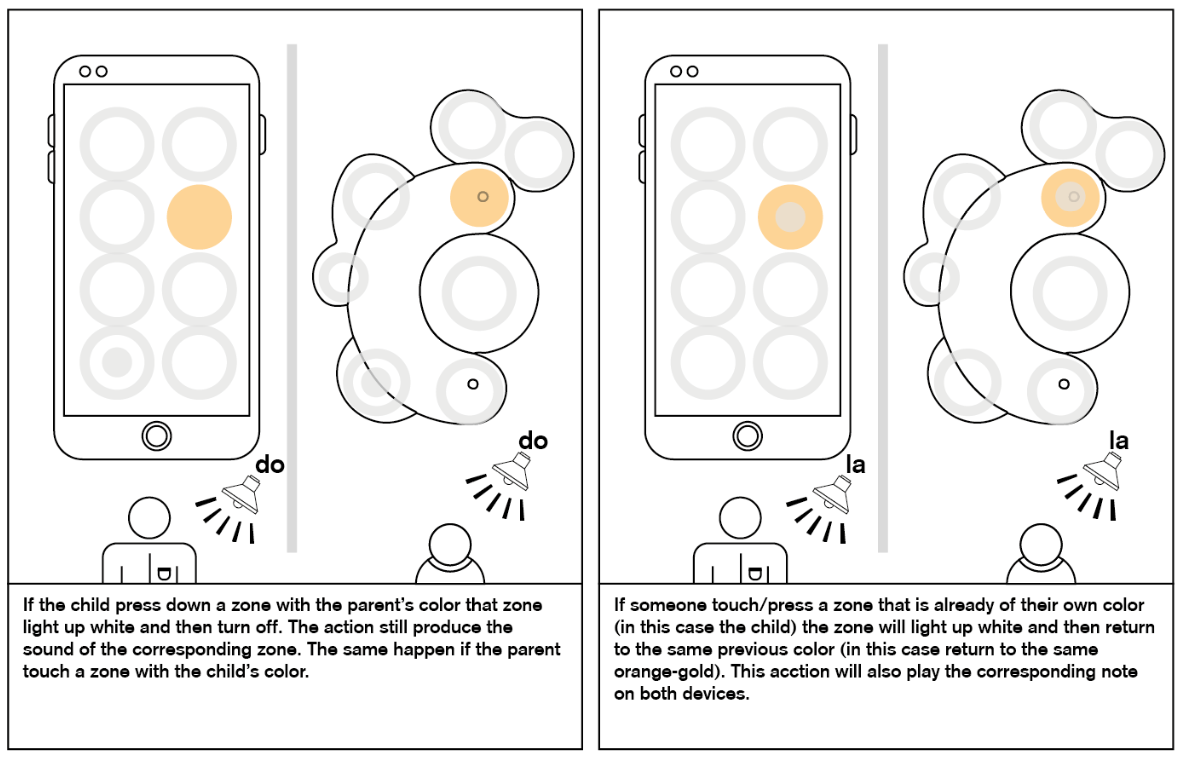
\includegraphics[scale=0.35]{images/FW/play_2.PNG}}\hfill
    \caption{Interaction design for child/parent game session } 
    \label{fig:game_id}
\end{figure}



\subsection{Work with ECAL designers}
\subsection{Business + Analysis of potential users + Customer journey}
\subsection{SHS research project and insights}